\section{Proof-of-Concept and Results}

\begin{frame}{Experimentation Setup}
  
  \begin{itemize}
  	\item We experiment on the SAE (synthetic) application whose minimum frequency to meet its RT requirements is known ($500$MHz).
  	\item We map SAE to a 2x2 instance of our manycore
	\item We perform clustering using the \textit{max-proc} criterion and $n = 4$.
	\item The nominal frequency of our platform is $2.5$GHz, which is also given as input to our framework. 
	\item By the last iteration, our framework found $500.4$MHz as the minimum frequency to meet the RT constraints on the platform. Since we cannot display the results for all iterations, we couple to show the last step and demonstrate how the found frequency meets the requirement of the application (the last frequency).
  \end{itemize}
  
\end{frame}


\begin{frame}
	
	\begin{itemize}
		\item The CPA method estimated the end-to-end iteration execution time of SAE based on the application graph and the WCET of the kernel operations. 
		
		\item Our scheduler has a WCET of $110$ kcycles, and our network driver has a WCET of $20$ kcycles. Tasks are scheduled once per iteration due to our PBRR implementation. The total iteration execution time, as pointed out by the CPA method, is $8.464.895$ cycles. 
		
		\item The actual RTL execution is $6.799.200$ cycles ($80\%$). The CPA method overestimates $\simeq 26\%$ of the actual CPU usage. However, the overestimation is \textit{acceptable} ($<30\%$) as the actual CPU usage stays below  $70\%$; a CPU usage over $70\%$ is often considered questionable~\cite{Ovaska:2011}.
		
	\end{itemize}
	

\end{frame}

\begin{frame}{}
    
    \vspace{-0.8em}
    \begin{table}[!ht]
    	\caption{Comparison of Execution time (CPU).}
    	\label{tab:results}
    	\centering
    	\resizebox{1\textwidth}{!}{%
    		\begin{tabular}{lrrrrr}
    			\toprule
    			\textbf{Cluster} & \textbf{Execution$^1$} & \textbf{Estimation$^2$} & \textbf{Difference} & \textbf{Diff. (\%)$^3$} & \textbf{Usage$^4$}\\
    			\cmidrule(lr){1-1}
    			\cmidrule(lr){2-2}
    			\cmidrule(lr){3-3}
    			\cmidrule(lr){4-4}
    			\cmidrule(lr){5-5}
    			\cmidrule(lr){6-6}
    			
    			\rowcolor{\rowcolordark} 
    			ABDF & $1,439,000$ & $1,819,300$ & $+380,300$ & $+26.428\%$ & $72.722\%$\\
    			
    			C & $801,300$ & $963,300$ & $+162.000$ & $+20.217\%$  & $38.532\%$\\
    			
    			\rowcolor{\rowcolordark} 
    			EHI & $2,174,500$ & $2,667,895$ & $+493,395$ &  $+22.690\%$  & $71.616\%$\\
    			
    			GJ & $2,384,400$ & $3,014,400$ & $+630.000$ & $+26.421\%$ & $86.980\%$\\     
    			
    			\bottomrule
    			\multicolumn{6}{p{9.5cm}}{\footnotesize{$^1$Execution time (RTL, cycles); $^2$CPA estimation; $^3$Execution time is $100\%$; $^4$DES.}}
    		\end{tabular}
    		
    	} % end of resize box
    \end{table}
    \vspace{-0.8em}
\end{frame}


\begin{frame}
	
	\begin{itemize}
		
		\item The framework captured the time that tasks finished during the DES simulation. As tasks implement the PREM and LET models, we assume that packets are injected at the same time they leave the CPU.
		
		\item Table~\ref{tab:flows} shows the characterization of flows, where $ph$ is the phase time (the period of scheduling interrupts), $pv$ is the \textit{phase} of the task, and $\psi = (ph \times pv)$. 
		
		\item A phase corresponds to the alignment of application execution to the scheduler tick. For instance, the SAE application cannot finish before the $4^{th}$ phase due to the critical path traverses 4 tasks in the application graph. This is a necessary step, as the DES simulation does not account for task dependency. Deadlines match the end of the phase of the receiving task.%GRAMMARLY-OK
				
	\end{itemize}
	
\end{frame}



\begin{frame}
	
	
	\vspace{-10 pt}
	\begin{table}[!ht]
		\caption{Characterization of flows for the SAE application.}
		\label{tab:flows}
		\centering
		\resizebox{0.8\textwidth}{!}{%
			\begin{tabular}{lrccrr}
				\toprule
				\textbf{Flow} & \textbf{MRT$^1$} & \textbf{S} & \textbf{D} & \textbf{Volume} & \textbf{Deadline}\\
				\cmidrule(lr){1-1}
				\cmidrule(lr){2-2}
				\cmidrule(lr){3-3}
				\cmidrule(lr){4-4}
				\cmidrule(lr){5-5}
				\cmidrule(lr){6-6}
				
				\rowcolor{\rowcolordark} $F_1$ & $285300 + \psi$ & A & C & $12300$ & $110000 +  \psi$\\
				$F_2$ & $1819300 + \psi$ & F & G & $67800$ & $110000 + \psi$\\
				\rowcolor{\rowcolordark} $F_3$ & $963300  + \psi$ & C & E & $12000$ & $110000 + \psi$\\
				$F_4$ & $1280700 + \psi$ & I & J & $56700$ & $1208800  + \psi$\\
				\rowcolor{\rowcolordark} $F_5$ & $1733700 + \psi$ & H & J & $89000$ & $1208800 + \psi$\\
				
				\bottomrule
				\multicolumn{6}{p{7cm}}{\footnotesize{(S) source task, (D) destination task, $^1$Minimum release time.}}
			\end{tabular}
			
		} % end of resize box
		\vspace{-8 pt}
	\end{table}	
	
\end{frame}



\begin{frame}
	\begin{itemize}
		\item In Figure~\ref{fig:phases}, we present the RTL simulation of our manycore running the SAE application at the minimum frequency of $500.4$MHz, obtained from our framework. The goal is to demonstrate that the application meets its RT requirements. 
		
		\item The hyperperiod of SAE is $20$ms, corresponding to 4 phases of $5$ms each, meeting the expected iteration time and iterations per second requirements. SAE receives stimuli from outside the system once per $5$ms, triggering $4$ instances of the application per $20ms$ (Task \textsc{a}). SAE returns results to outside the system via Task \textsc{j}. 
		
		\item The $3^{\text{rd}}$ instance of the application (pink) has additional $1.457$ms in its iteration time, related to the scheduling of Task \textsc{i}; the task executes two iterations at once due to two packets received in the phase time, delaying Task \textsc{j}. Nevertheless, Task \textsc{j} meets its deadlines for all instances of SAE, for an iteration time of $16,820$ms for the $1^{\text{st}}$, $2^{\text{nd}}$ and $3^{\text{th}}$ instances, and $18.277$ms for the $3^{\text{rd}}$ instance.
	\end{itemize}
\end{frame}


\begin{frame}
	\begin{figure}[!ht]
		\centerline{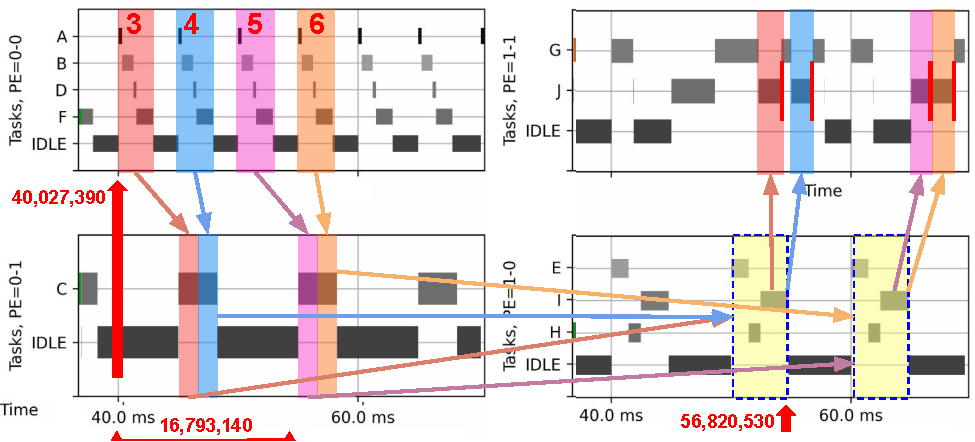
\includegraphics[width=0.8\columnwidth]{fig/results.pdf}}
		\caption{Interaction of tasks of the SAE application during RTL simulation. Rectangles with the same color represent tasks in the same iteration (instances). Arrows indicate the direction of the communication. The yellow rectangle represents a phase overlapping.}
		\vspace{-16 pt}
		\label{fig:phases}
	\end{figure}
\end{frame}